\section{Operational Design Domain (ODD) limits}\label{sec:odd}
\subsection{Problem}
Most deployed autonomous driving systems are specified to work only inside an \emph{Operational Design Domain}: the operating conditions (road type, geography, lighting, weather, traffic) under which the system is designed to function~\cite{sae}. In practice this means strictly mapped, geofenced urban areas with structured roads, and the system is expected to hand over or stop when conditions leave that envelope (a ``minimal risk condition''). The concept paper's premise is that such systems work safely inside their mapped boundaries and fail outside them. We take that premise as the working hypothesis and do \emph{not} verify claims about any particular company's system. The questions studied here are quantitative:
\begin{enumerate}\setlength\itemsep{0pt}
\item How much of a real, dense, unstructured night-time Indian street drive would fall \emph{inside} a structured-urban ODD?
\item How does the social planner behave as conditions leave the ODD, and what are the options: refuse to operate (strict ODD), carry on unaware, or adapt?
\end{enumerate}

\subsection{ODD specification and runtime monitor}
We define an illustrative ODD with five attributes, each measured per frame from the clip by a classical-CV proxy (Table~\ref{tab:oddspec}). The thresholds are \emph{assumed} (they stand for a structured, lit, marked-lane, moderate-traffic domain) and are varied in a sensitivity analysis. Each attribute has a quality $q_k\in[0,1]$ ($1$ when inside the specification, falling linearly to $0$ at twice the threshold excursion), smoothed over about 1\,s. The \emph{ODD monitor} outputs $q=\min_k q_k$ (weakest link). Two variants are used: $q_{\text{all}}$ over all five attributes (strict ODD) and $q_{\text{perc}}$ over the four attributes that matter for detecting other road users (lane markings excluded).

\begin{table}[H]\centering\small
\begin{tabular}{p{0.2\linewidth}p{0.5\linewidth}p{0.2\linewidth}}\toprule
Attribute & Video proxy & Inside if\\\midrule
Lane markings & total length of near-diagonal Hough lines in the road region, as a fraction of image width & $\ge 0.15$\\
Lighting & fraction of road-region pixels with luma $<30$ & $\le 0.12$\\
Glare & fraction of road-region pixels saturated ($\ge250$) & $\le 0.02$\\
Traffic complexity & independent-motion fraction (Section~2) & $\le 0.15$\\
Image sharpness & variance of the Laplacian of the road region & $\ge 800$\\\bottomrule
\end{tabular}\caption{Illustrative ODD attributes (thresholds assumed).}\label{tab:oddspec}\end{table}

\subsection{How much of the clip is inside the ODD?}
Over the 199.7\,s of driving, \textbf{only 6.1\% of the time satisfies all five attributes}, and 17.2\% satisfies the four attributes other than lane markings. After a 1\,s debounce the status exits the ODD 2.4 times per minute, and the mean uninterrupted time inside is about 1\,s, so a strict ODD would be unusable rather than merely often violated. The attributes violated most are lane markings (74\% of driving time) and traffic complexity (64\%), followed by lighting (23\%), sharpness (19\%) and glare (15\%) (Figures~\ref{fig:oddframes}--\ref{fig:oddviol}).

\begin{figure}[H]\centering
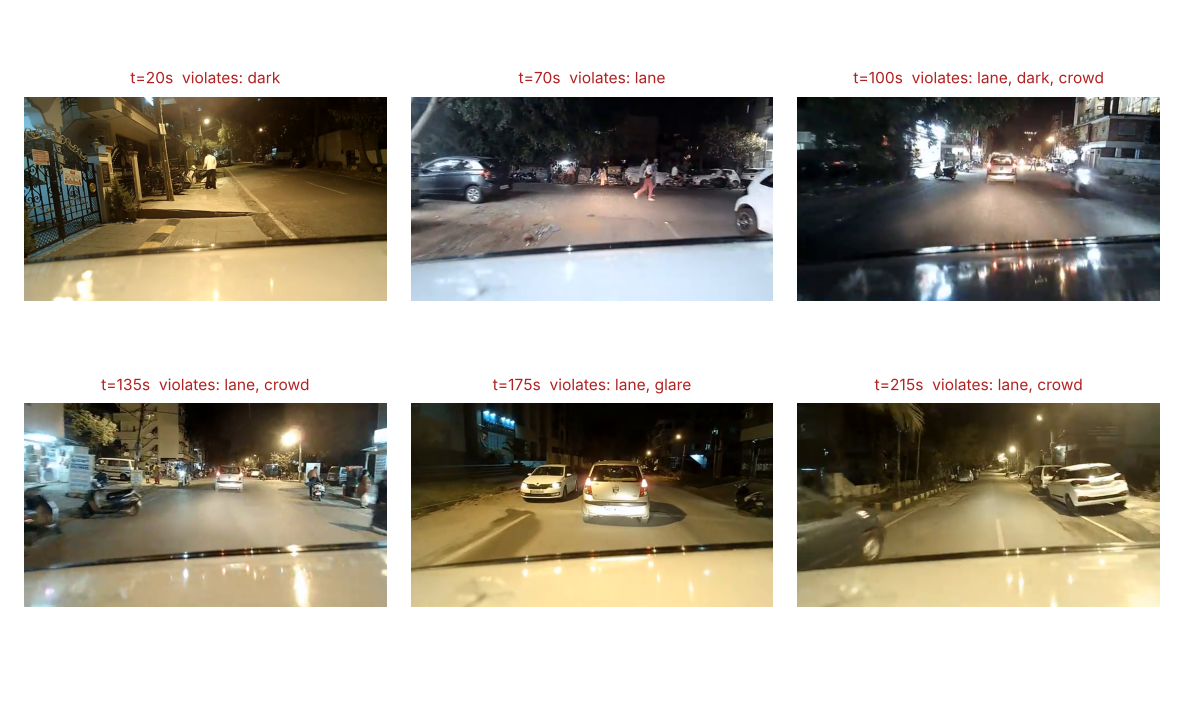
\includegraphics[width=\linewidth]{odd_frames.png}
\caption{Six frames labelled with the ODD attributes they violate. Note t=215\,s: dashed lane markings are visible but the lane proxy flags a violation (see caveat below).}\label{fig:oddframes}
\end{figure}
\begin{figure}[H]\centering
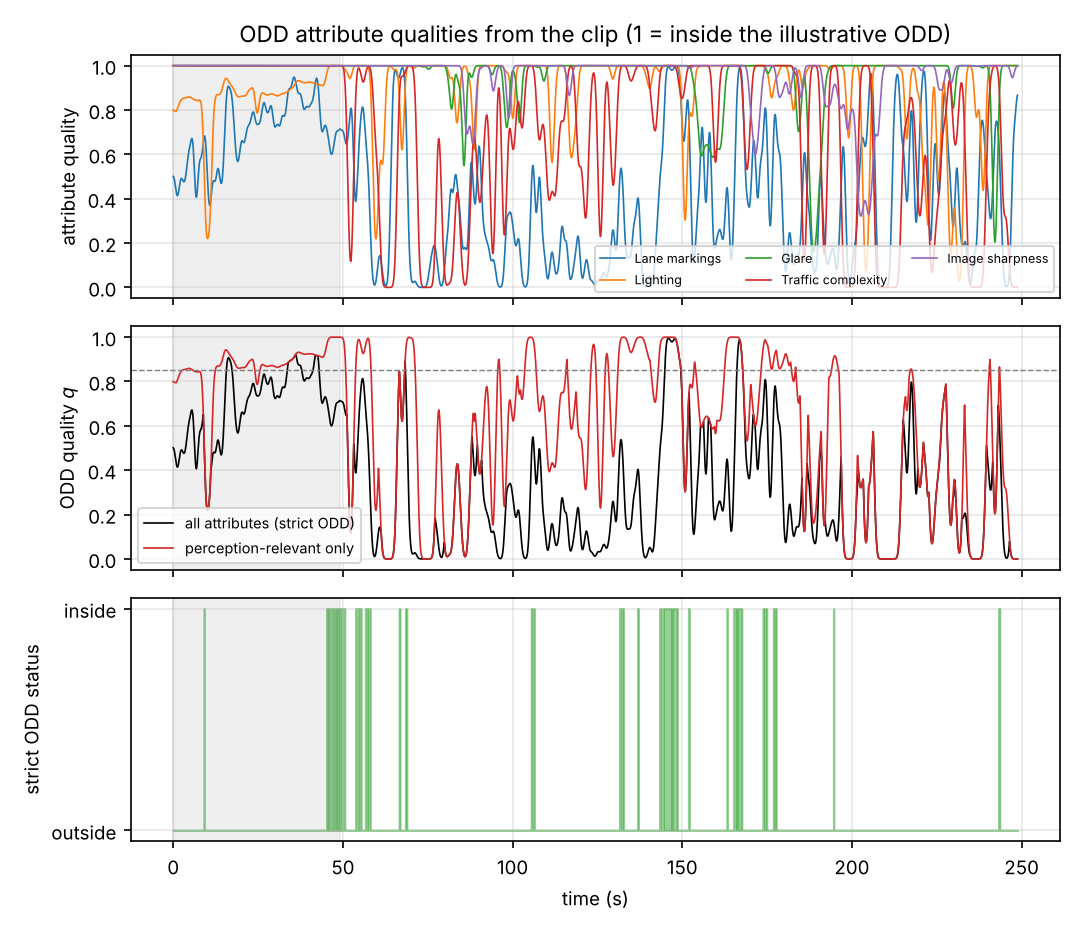
\includegraphics[width=\linewidth]{odd_timeline.png}
\caption{Attribute qualities, monitor output $q$ and strict ODD status through the clip (grey = parked prefix). The dashed line marks $q=0.85$, the strict-ODD disengagement threshold used later.}\label{fig:oddtl}
\end{figure}
\begin{figure}[H]\centering
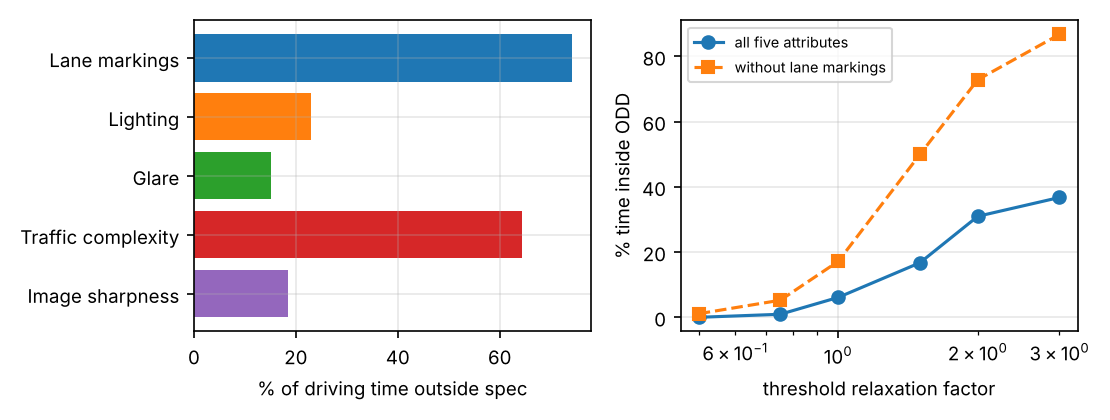
\includegraphics[width=\linewidth]{odd_violations.png}
\caption{Left: share of driving time each attribute is outside its specification. Right: time inside the ODD as all thresholds are relaxed by a common factor (log scale).}\label{fig:oddviol}
\end{figure}

\begin{table}[H]\centering\small
\begin{tabular}{lrrrrrr}\toprule
Threshold relaxation factor & 0.5 & 0.75 & 1 & 1.5 & 2 & 3\\\midrule
Inside ODD, all five attributes (\%) & 0.0 & 0.9 & 6.1 & 16.7 & 31.0 & 36.7\\
Inside ODD, without lane markings (\%) & 1.1 & 5.2 & 17.2 & 49.9 & 72.9 & 86.7\\\bottomrule
\end{tabular}\caption{Sensitivity of ODD conformance to the assumed thresholds.}\end{table}

\paragraph{Descriptive comparison with the human driver.} In the 6\% of time inside the ODD the human driver averaged 7.1\,m/s with RMS jerk 1.79\,m/s$^3$; outside, 8.2\,m/s and 2.30\,m/s$^3$. With so little time inside, this is a description, not evidence that conditions outside the ODD change driver behaviour.

\paragraph{Caveat: the proxies lean towards violation.} The lane proxy misses dashed markings that are visible in the frames (t=215\,s in Figure~\ref{fig:oddframes}), and the traffic-complexity proxy is inflated by parallax from near structures (Section~2). The 6\% figure should therefore be read as a lower bound. However, relaxing every threshold by a factor of two still leaves the full ODD satisfied for only 31\% of the time (73\% without lane markings), so the qualitative conclusion, that this environment is mostly outside a structured ODD, is robust to the proxy choice.

\subsection{Planner behaviour as conditions leave the ODD}
\paragraph{Degradation model (assumed).} We let a scene-level ODD quality $q$ degrade the ego's perception of opponents: position noise $\sigma_d=0.3+3(1-q)$\,m, speed noise $\sigma_v=0.1+(1-q)$\,m/s, per-step miss probability $0.35(1-q)^2$ and latency $0.5(1-q)$\,s. The monitor observes $\hat q=q+\mathcal N(0,0.05^2)$. This mapping is not fitted to any sensor.

\paragraph{Policies.}
\begin{description}\setlength\itemsep{0pt}
\item[Strict-ODD (geofence-style).] Runs the social planner if $\hat q\ge0.85$, otherwise disengages (no trip). We assume the resulting minimal-risk stop is perfectly safe, which favours this policy on safety.
\item[ODD-unaware.] Runs the social planner at any $q$.
\item[ODD-aware: persistence.] Keeps a track of a briefly undetected opponent for up to 1.5\,s, extrapolating at constant velocity; disengages only if $\hat q<0.15$.
\item[ODD-aware: persistence + margins.] Additionally inflates the safety-shield margins by $1+1.5(1-\hat q)$.
\end{description}
Experiments use the medium-density scenario. A controlled sweep covers $q\in\{1.0,0.9,\dots,0.1\}$ (300 episodes per point and policy). A video-conditioned run draws $q$ from the empirical distribution of $q_{\text{perc}}$ over the driving portion of the clip (median 0.61, quartiles 0.26 and 0.85) with 900 episodes per policy.

\begin{figure}[H]\centering
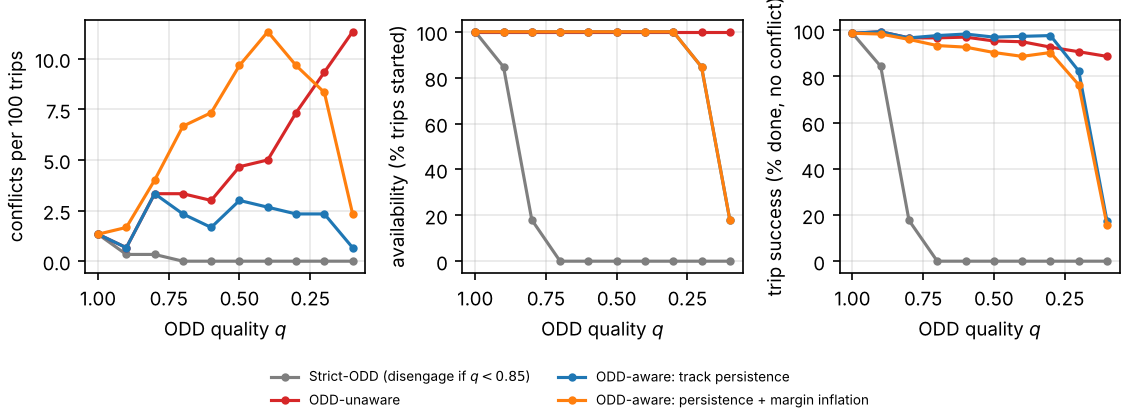
\includegraphics[width=\linewidth]{odd_sweep.png}
\caption{Conflicts, availability and trip success against ODD quality $q$ (note the reversed axis). Points are noisy (300 episodes each).}\label{fig:oddsweep}
\end{figure}

\begin{table}[H]\centering\footnotesize
\resizebox{\linewidth}{!}{\begin{tabular}{lrrrrr}
\toprule
Policy & Avail. \% & Coll. \% (of all) & Coll. \% (if started) & Success \% & Delay (s) \\
\midrule
Strict-ODD (geofence-style) & 25.3 & 0.33 & 1.32 & 25.0 & 4.4 \\
ODD-unaware & 100.0 & 5.00 & 5.00 & 95.0 & 3.6 \\
ODD-aware: persistence & 81.0 & 2.00 & 2.47 & 79.0 & 4.7 \\
ODD-aware: persistence + margins & 81.6 & 4.44 & 5.45 & 77.1 & 11.5 \\
\bottomrule
\end{tabular}
}
\caption{Video-conditioned results ($q$ sampled from the clip's $q_{\text{perc}}$ distribution, 900 episodes per policy). ``Avail.'' = trips started; ``Success'' = trips completed without conflict; delay is over started trips.}\label{tab:oddvideo}\end{table}

\paragraph{Findings.}
\begin{itemize}\setlength\itemsep{1pt}
\item \textbf{The ODD is the binding constraint.} With conditions like the clip's, the strict-ODD policy would start only 25\% of trips; below $q=0.85$ it starts none (Figure~\ref{fig:oddsweep}, middle). Its safety is excellent (0.3\% conflicts over all trips), but this partly reflects trips that never happen.
\item \textbf{Operating unaware is unsafe, and increasingly so.} Conflicts rise from 1.3\% at $q=1$ to 11\% at $q=0.1$; under the clip's conditions the unaware planner has 5.0\% conflicts.
\item \textbf{Cheap robustness helps.} Track persistence keeps conflicts at roughly 1--3\% across $q$ from 0.2 to 0.9 and cuts the video-conditioned conflict rate from 5.0\% to 2.0\% (2.5\% of started trips) at 81\% availability and a small delay increase (4.7\,s versus 3.6\,s unaware).
\item \textbf{Being more conservative can backfire.} Adding margin inflation raised delay to 11.5\,s and conflicts to 4.4\% (5.5\% of started trips), worse than persistence alone and, at mid $q$, worse than doing nothing (up to 11\% around $q=0.4$). In an isolation test at $q=0.8$ and $0.5$, margin inflation without persistence gave 5.7\% and 18.7\% conflicts. A plausible mechanism, not verified here, is that longer waits give courteous opponents time to stop, lose patience and restart, which lengthens exposure; it echoes the hesitation effect seen in the politeness sweep.
\end{itemize}
Together these results support a graded view of the ODD (strict boundary, degraded-but-monitored operation, minimal-risk fallback) over a hard geofence, but only under the assumed degradation model; they do not show that any particular adaptation would work on a real vehicle.
